\chapter{Effect of horizontal resolution on simulated larval retention patterns}\label{Chap2}

\section{Introduction}\label{Chap2Intro}

Interest in the early life stages of marine organisms has increased \citep{Stra1993,Haven1995,Levi2006,GawaMoni2007,CoweSpon2009} in particular for understanding larval transport and dispersal patterns \citep{Youn1995,GreeMayp2015,Leis2021} due to their key role in the ecology of marine organisms \citep{MoseSmit1993} and potential usefulness in decision making for the management of \acrfull{mpa} \citep{DaloBogd2015}. Many marine species have pelagic early life stages in their life cycle \citep{Haven1995}. This phase of locomotion is essentially driven by ocean currents and species-specific vertical behaviours \citep{Levi1990,CowePari2006,DaloBogd2015}.\\

In the case of sessile organisms, such as scallops and corals, concepts such as larval transport, larval dispersal and population connectivity have been formally defined \citep{PineHare2007}. Hence, \textbf{larval transport} is the horizontal translocation of a larva between points $X_{1}Y_{1}$, and $X_{2}Y_{2}$, where $X$ and $Y$ are the horizontal axes, perpendicular and parallel to the coastline respectively (to simplify, this definition ignores the vertical axis $Z$). On the other hand, \textbf{larval dispersal} refers to the spread of larvae from a spawning source to a settlement site (a geographic point from which the adult will have limited or no mobility). We note that larval transport is a component of larval dispersal (Fig. \ref{Chap2LarvalTransport}). Finally, \textbf{population connectivity} is the exchange of individuals among geographically separated subpopulations. We note that larval dispersal is a component of population connectivity, and therefore larval transport too. In the case of pelagic or demersal organisms such as fish, these general concepts also apply but the movement of adults is also an important component of population connectivity.\\

\begin{figure}[ht]
	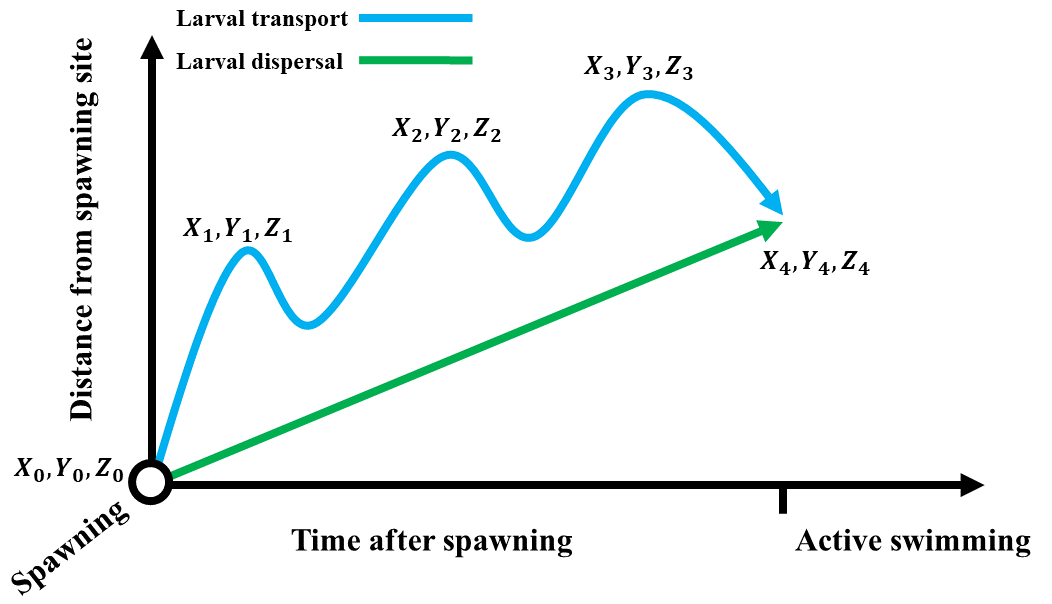
\includegraphics[width=1.0\textwidth]{figures/Chap2LarvalTransport.png}
	\centering
	\caption{Schematic representation of larval transport and larval dispersal processes. Note that the sum of the larval transport distance is greater than the dispersal distance. All locations ($X_{n},Y_{n},Z_{n}$) are pelagic.}
	\label{Chap2LarvalTransport}
\end{figure}

During larval transport, organisms are dragged by currents and depend on environmental conditions to survive, whether temperature and/or food \citep{NocrShaw1984}, and currents may allow larvae to match their food source location \citep{CuryRoy1989}. It is in this context that larval drift models, which allow tracking the trajectory of eggs and larvae through a virtual environment, are a fundamental tool for understanding the transport patterns of different species. However, before interpret modelling results it is recommended to perform a sensitivity analysis to test the robustness of these results \citep{PeckHufn2012,SimoSieg2013}. Sensitivity analysis can be understood as the manner in which model behaviour depends on model parametrization or as the variation of the response variable as a function of a change in a model parameter \citep{Hamb1994,Inga2008}. In larval drift models, results may be sensitive to the number of released particles \citep{SimoSieg2013}, to lethal temperature \citep{BrocLett2008}, to wind frequency forcing \citep{FlorTam2019}, to the spatial resolution of the forcing currents \citep{GaraKapl2014}, etc. Here we will also focus our sensitivity analysis on spatial resolution.\\

\clearpage

\section{Methods}\label{Chap2Meth}

An \acrfull{ibm} simulates populations and communities by following individuals and their properties \citep{DeanGrim2014}. As a base, this \acrshort{ibm}, that we will use from here on, is a lagrangian tool called \href{https://ichthyop.org/}{Ichthyop} – Lagrangian tool for simulating ichthyoplankton dynamics, version 3.2 \citep{LettVerl2008}. In general, a protocol designed for this type of \acrshort{ibm} approach will be followed \citep{GrimBerg2006,GrimBerg2010}. In the following chapters, the complexity of the model will be increased by adding specific modules for new processes.\\

\subsection{Purpose}\label{Chap2MethPurp}

To evaluate the impact of spatial resolution, bathymetry and coastline behaviour on transport and retention patterns of generic particles in the coastal zone off Peru.\\

\subsection{Entities and state variables}\label{Chap2MethEnti}

The model included two types of entities: the environment and the individuals (virtual particles). The environment was represented by stored hydrodynamic simulations from the \acrlong{croco} (\href{https://www.croco-ocean.org/}{CROCO}, \cite{HiltAucl2020,ShchMcwi2005}) providing the forcing state variables: ocean current velocities ($ms^{-1}$), over the \acrshort{nhcs}. Individuals were characterized by the following state variables: age ($d$), location in 3D (longitude, latitude and depth).\\

Fig. \ref{Chap2SpawningZone} xshows the three different \acrshort{croco} configurations with contrasted grid size and bathymetry were used, in order to evaluate the model sensitivity to hydrodynamic resolution (Table \ref{TabSimus}). The first configuration (D01) extends from 22 °S to 5 °N in latitude and from 96 °W to 70 °W in longitude, with a horizontal resolution of $\sim$10 km and 32 vertical levels. The bathymetry comes from the STRM30 dataset \citep{BeckSand2009}. It was interpolated on the model grid and smoothed in order to reduce errors in the horizontal pressure gradient. The second configuration (D02) extends from 20 ºS to 5 ºS with a horizontal resolution of $\sim$2 km and 42 vertical levels. The D02 domain is embedded in the D01 domain, through an offline nesting procedure (``roms2roms''; \cite{MasoMole2010}). We used two different bathymetries for the D02 domain: one interpolated from the D01 bathymetry (i.e., similar to the D01 bathymetry) and one interpolated directly from the STRM30 dataset. Note that consequently the former is smoother than the latter, so in the following we call them D02s and D02r, respectively.\\

\begin{figure}[ht]
	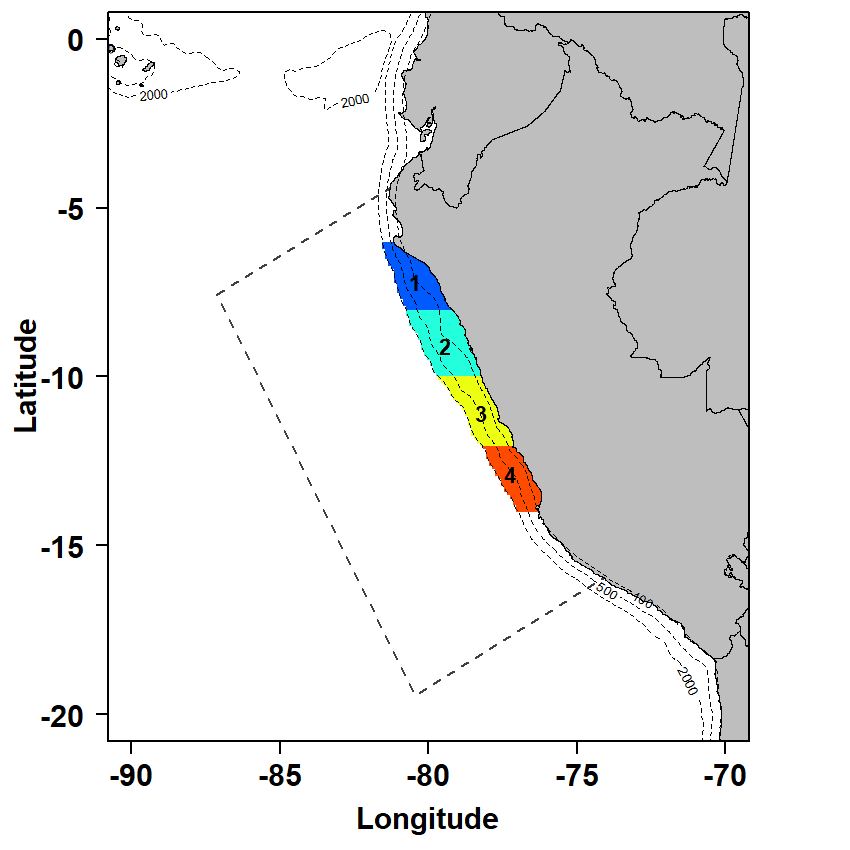
\includegraphics[width=1.0\textwidth]{figures/Chap2SpawningZone.png}
	\centering
	\caption{Domain of \acrshort{ibm} model study area at 10 km of spatial resolution (D01). Dotted rectangle represents the nested model domains (D02s, D02s) at 2 km resolution used for spatial resolution test. Spawning areas (1 to 4) are every 2 degrees of latitude between 6º – 14º S. Three isobaths (100 m, 500 m and 2000 m) are shown.}
	\label{Chap2SpawningZone}
\end{figure}

%\begin{landscape}
\begin{table}
\centering
\begin{tabular}{c|c|c|c}
\hline
                           & \textbf{Sim 1} & \textbf{Sim 2}          & \textbf{Sim 3} \\
\hline
Configuration domain       & D01            & D02s                    & D02r           \\
Bathymetry                 & STRM30         & Interpolated from Sim 1 & STRM30         \\
Forcing type               & Physical       & Physical                & Physical       \\
Horizontal grid resolution & 10 km          & 2 km                    & 2 km           \\
CROCO configuration        & 22ºS to 5ºN    & 20ºS to 5ºS             & 20ºS to 5ºS    \\
Latitudinal spawning range & 6ºS - 14ºS     & 6ºS - 14ºS              & 6ºS - 14ºS     \\
Coastline behavior &
  \begin{tabular}[c]{@{}c@{}}beaching,\\ bouncing,\\ standstill\end{tabular} &
  \begin{tabular}[c]{@{}c@{}}beaching,\\ bouncing,\\ standstill\end{tabular} &
  \begin{tabular}[c]{@{}c@{}}beaching,\\ bouncing,\\ standstill\end{tabular}
\end{tabular}
\caption{Summary of simulations in Chapter \ref{Chap2} performed to sensitivity analysis. This table list all parameters that differ between simulations.}
\label{TabSimus}
\end{table}
%\end{landscape}

The three configurations were used to obtain quasi-equilibrium solutions, forced by monthly climatologies (over the period 2008-2015) at their surface and lateral boundaries. They all used the same atmospheric forcing fields. The wind stress was computed from a monthly climatology of the \acrlong{ascat} (\href{https://www.ospo.noaa.gov/Products/atmosphere/ascat/}{ASCAT}, 1/4° gridded product). Other atmospheric fluxes (shortwave heat fluxes and freshwater fluxes) come from the \acrlong{coads} \href{https://repository.library.noaa.gov/view/noaa/49337}{COADS} monthly climatology \citep{DasiYoun1994}. Model \acrfull{sst} was restored to observed climatological monthly \acrshort{sst} derived from the merged multi-sensor OSTIA product \citep{DonlMart2012} following the methodology of \citep{BarnSief1995}. Open boundary conditions for the D01 domain were derived from a monthly climatology of the \href{https://www.mercator-ocean.eu/en/ocean-science/glorys/}{GLORYS2V4} reanalysis [1/4° horizontal resolution; \citep{FerrPare2012}] for temperature, salinity, zonal and meridional current velocity components and sea-level height. Climatological simulations were run for 10 years, the first 4 years being considered as a spin-up. In the present study, the last three years were used to force \gls{ich}.\\

\subsection{Process overview and scheduling}\label{Chap2MethProc}

Virtual individuals were released in the physical environment according to a determined spatial (area, depth and bathymetry) and temporal (month and frequency) releasing strategy that constituted the initial conditions (section \ref{Chap2MethInit}). For each time step (2 hours) each egg or larva was passively transported by the 3D current fields and was then tested for recruitment.\\

\subsection{Design concepts}\label{Chap2MethDesi}

\begin{itemize}

\item Stochasticity: Individuals were initially randomly distributed over the Peruvian continental shelf. We chose the number of individuals released (5 000) such that the variability of simulated recruitment between three replicates of the same simulation was negligible.\\

\item Coastline behavior: One of the utilities of \gls{ich} is the option to use different response configurations of a particle when faced with the decision of what to do when it touches the land boundary (coastline). We tested three types of coastline behaviors: 1) \textbf{BEACHING}: \gls{ich} does move the particle inland but ``kill'' it. From now onward the particle is out of the simulation. 2) \textbf{BOUNCING}: the coastline acts as a billard edge and the particle will bounce as a billard ball in the events that the move would take it beyond the coastline. The particle bounces back as much as it would penetrate inland and 3) \textbf{STANDSTILL}: the particle gives up on the move that would take it inland and just wait until next time step for trying another move.\\

\item Observation: After 30 days of drift, each particle was tested to see if it was within the continental shelf and was considered ``retained'' or ``non-retained''. From now on, we will call \gls{cri1}, referring ``retention'' as a criterion for larval recruitment.\\

\end{itemize}

\subsection{Initialization}\label{Chap2MethInit}

In each simulation, individuals were released randomly along the coastal release area each month at days 1, 10 and 20, during the three climatological years used.\\

Release area (Fig. \ref{Chap2SpawningZone}) was defined between latitudes 6°S and 14°S, depths 0 m to 45 m and from the coast to bathymetry contour 2000 m. This area was further splitted into different subdomains for the simulations post-processing and analysis (released depth ranges 0-15 m, 15-30 m and 30-45 m; cross-shore extension delimited by isobaths 0-100 m, 100-500 m, 500-2000 m).\\

\subsection{Sub-models}\label{Chap2MethSubMod}

\begin{itemize}

\item Transport: To simulate particle transport, virtual individuals were advected using a trilinear interpolation scheme of the velocity fields derived from \acrshort{croco}, in time and space, and using a forward Euler numerical scheme with horizontal diffusion following \cite{PeliMarc2007}.\\

\item Retention: We considered one age-criterion for recruitment, hereafter referred to as \gls{cri1}. An individual was considered as ``recruited'' if it was within the coastal zone (offshore limit: the 2000 m isobath) at age 30 days.\\

\end{itemize}

\subsection{Simulations and sensitivity analysis}\label{Chap2MethSimSens}

From this chapter onwards, each drift simulation will be listed under the name ``\textbf{sim \#}'', for example, in the text, saying ``sim 1'', will be equivalent to saying ``simulation 1''. Details of each simulation will be detailed in a table in its corresponding chapter.\\

Three simulations were performed in order to explore the model sensitivity to different environmental forcing fields (Table \ref{TabSimus}). In order to fit the spatial extent of the 2 km grid, individuals release was constrained in the coastal area between 6 ºS and 14 ºS (Fig. \ref{Chap2SpawningZone}, dotted box) for all three simulations. Larval recruitment was calculated at 30 days.\\

\clearpage

\section{Results}\label{Chap2Resu}

Globally, simulation 1 (D01), simulation 2 (D02s) and simulation 3 (D02r) showed no significant differences (Fig. \ref{Chap2Recruitment3bars}). As all simulations were run with interannual forcing, no differences in recruitment rates were observed in the 3 years of simulation and were also not impacted by the frequency of release (not shown).\\

\begin{figure}[ht]
	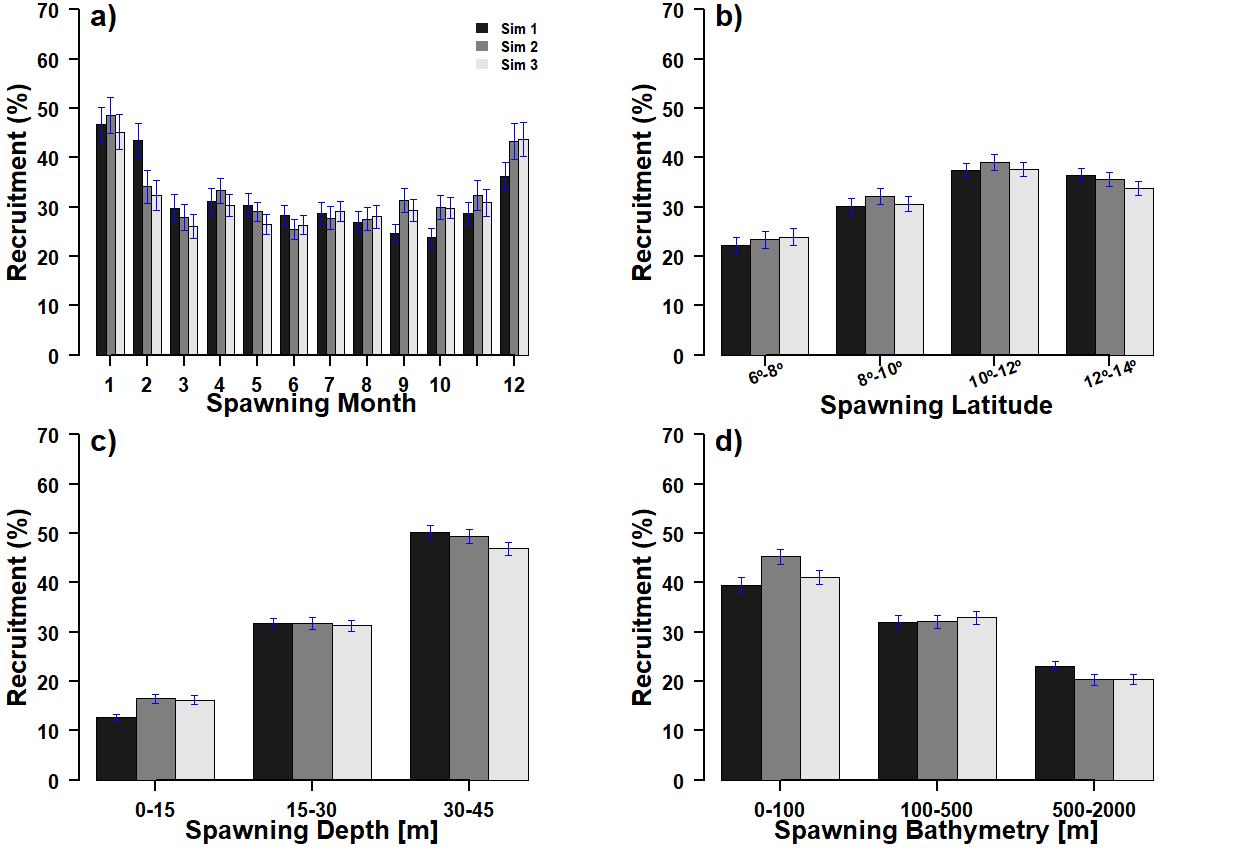
\includegraphics[width=1.0\textwidth]{figures/Chap2Recruitment3bars.png}
	\centering
	\caption{Percentage of recruited larvae of Peruvian anchovy obtained for different (a) spawning months, (b) spawning latitudes, (c) spawning depths, and (d) isobaths delimiting spawning areas horizontally, for three simulations using forcing fields at different spatial resolution (Sim 1 in black, Sim 2 in dark grey, Sim 3 in light gray; see Table \ref{TabSimus} for details on simulations characteristics). Blue arrows represent confidence interval (95 \%).}
	\label{Chap2Recruitment3bars}
\end{figure}

Since spatial resolution is not a factor that significantly affected retention rates, the results of the 3 simulations were combined and an ANOVA (Table \ref{TabAnovaSimus}) was applied to evaluate which of the other factors (release month, release latitude, release depth and release bathymetry) had the greatest impact. Release depth explained 30.11 \% of the variance and showed a direct relationship between release depth and retention rate, with higher values when the particles were released deeper (30 - 45 m) and lower values when they were released near the surface (0 - 15 m) (Fig. \ref{Chap2Recruitment3bars}c). Release bathymetry explained 12.95 \% of the variance, with the highest retention rates in the area closest to the coast (0 - 100 m) than those released offshore (100 - 500 m, 500 - 2000 m) (Fig. \ref{Chap2Recruitment3bars}d). Release month explained only 5.56 \% of the variance and showed seasonal variability with the summer months having the highest retention rate (Fig. \ref{Chap2Recruitment3bars}a). Finally, release latitude explained 4.58 \% of the variance and the zone between 10 - 12 ºS was the major latitudinal retention zone (Fig. \ref{Chap2Recruitment3bars}b).\\

\begin{landscape}
\begin{table}
\begin{tabular}{c|r|r|r|r|r|r}
\hline
 &
  \multicolumn{1}{c|}{\textbf{Df}} &
  \multicolumn{1}{c|}{\textbf{Sum Sq}} &
  \multicolumn{1}{c|}{\textbf{Mean Sq}} &
  \multicolumn{1}{c|}{\textbf{F value}} &
  \multicolumn{1}{c|}{\textbf{Pr (\textgreater{}F)}} &
  \multicolumn{1}{c}{\textbf{\% Exp}} \\
\hline
Year                  & 2     & 445.15     & 222.57     & 1.67    & 0.1883824  & 0.006  \\
Month                 & 11    & 402974.67  & 36634.06   & 274.79  & 0          & 5.567  \\
Depth                 & 2     & 2179965.33 & 1089982.67 & 8175.98 & 0          & 30.114 \\
Bathymetry            & 2     & 937366.31  & 468683.15  & 3515.60 & 0          & 12.949 \\
Latitude              & 3     & 331526.69  & 110508.90  & 828.93  & 0          & 4.580  \\
Year x Month          & 22    & 10599.92   & 481.81     & 3.61    & 2.11E-08   & 0.146  \\
Year x Depth          & 4     & 645.77     & 161.44     & 1.21    & 0.30375276 & 0.009  \\
Year x Bathymetry     & 4     & 2448.21    & 612.05     & 4.59    & 0.0010536  & 0.034  \\
Year x Latitude       & 6     & 17687.31   & 2947.88    & 22.11   & 5.02E-26   & 0.244  \\
Month x Depth         & 22    & 795678.29  & 36167.20   & 271.29  & 0          & 10.991 \\
Month x Bathymetry    & 22    & 111246.09  & 5056.64    & 37.93   & 2.63E-156  & 1.537  \\
Month x Latitude      & 33    & 526941.97  & 15967.94   & 119.78  & 0          & 7.279  \\
Depth x Bathymetry    & 4     & 49715.80   & 12428.95   & 93.23   & 3.67E-78   & 0.687  \\
Depth x Latitude      & 6     & 54521.66   & 9086.94    & 68.16   & 1.07E-83   & 0.753  \\
Bathymetry x Latitude & 6     & 282366.47  & 47061.08   & 353.01  & 0          & 3.901  \\
Residuals             & 11514 & 1534992.47 & 133.32     & -       & -          & 21.204
\end{tabular}
\caption{ANOVA of retention rates for simulation 1 (D01), simulation 2 (D02s) and simulation 3 (D02r) combined.}
\label{TabAnovaSimus}
\end{table}
\end{landscape}

Release depth had the highest and most significant effect on all 3 simulations affecting the seasonal pattern (Fig. \ref{Chap2Recruitment3sim3depth}). Particles released near the surface (0-15 m, Fig. \ref{Chap2Recruitment3sim3depth} a, d, g) showed a seasonal pattern favoring retention in the winter months, while this pattern reverses as release depth increases (15 - 30 m, Fig. \ref{Chap2Recruitment3sim3depth} b, e, h; 30 - 45 m, c, f, i).\\

\begin{figure}[ht]
	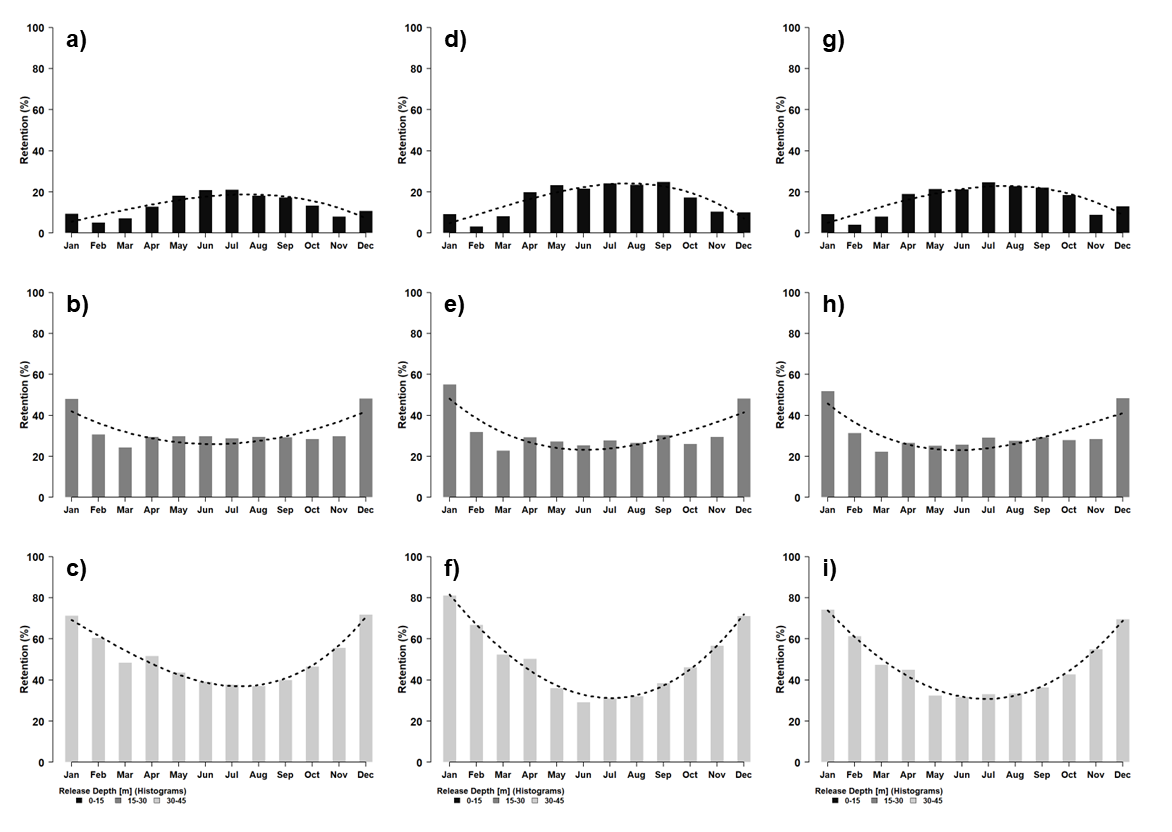
\includegraphics[width=1.0\textwidth]{figures/Chap2Recruitment3sim3depth.png}
	\centering
	\caption{Particle retention rates off Peru using 3 different physical forcing configurations (D01, a,b,c; D02s, d,e,f; D02r, g,h,i) and three release depths (0 – 15 m, 15 - 30 m and 30 - 45 m).}
	\label{Chap2Recruitment3sim3depth}
\end{figure}

Fig. \ref{Chap2SpatialVariation} showed that retention rates between 10\textdegree S - 12\textdegree S remained constant throughout the year in the 3 simulations. The northern zone between 6\textdegree S - 10\textdegree S showed seasonal variability with higher retention values in summer and accented values in January and February in simulation 2 (D02s).\\

\begin{center}
\begin{figure}[ht]
	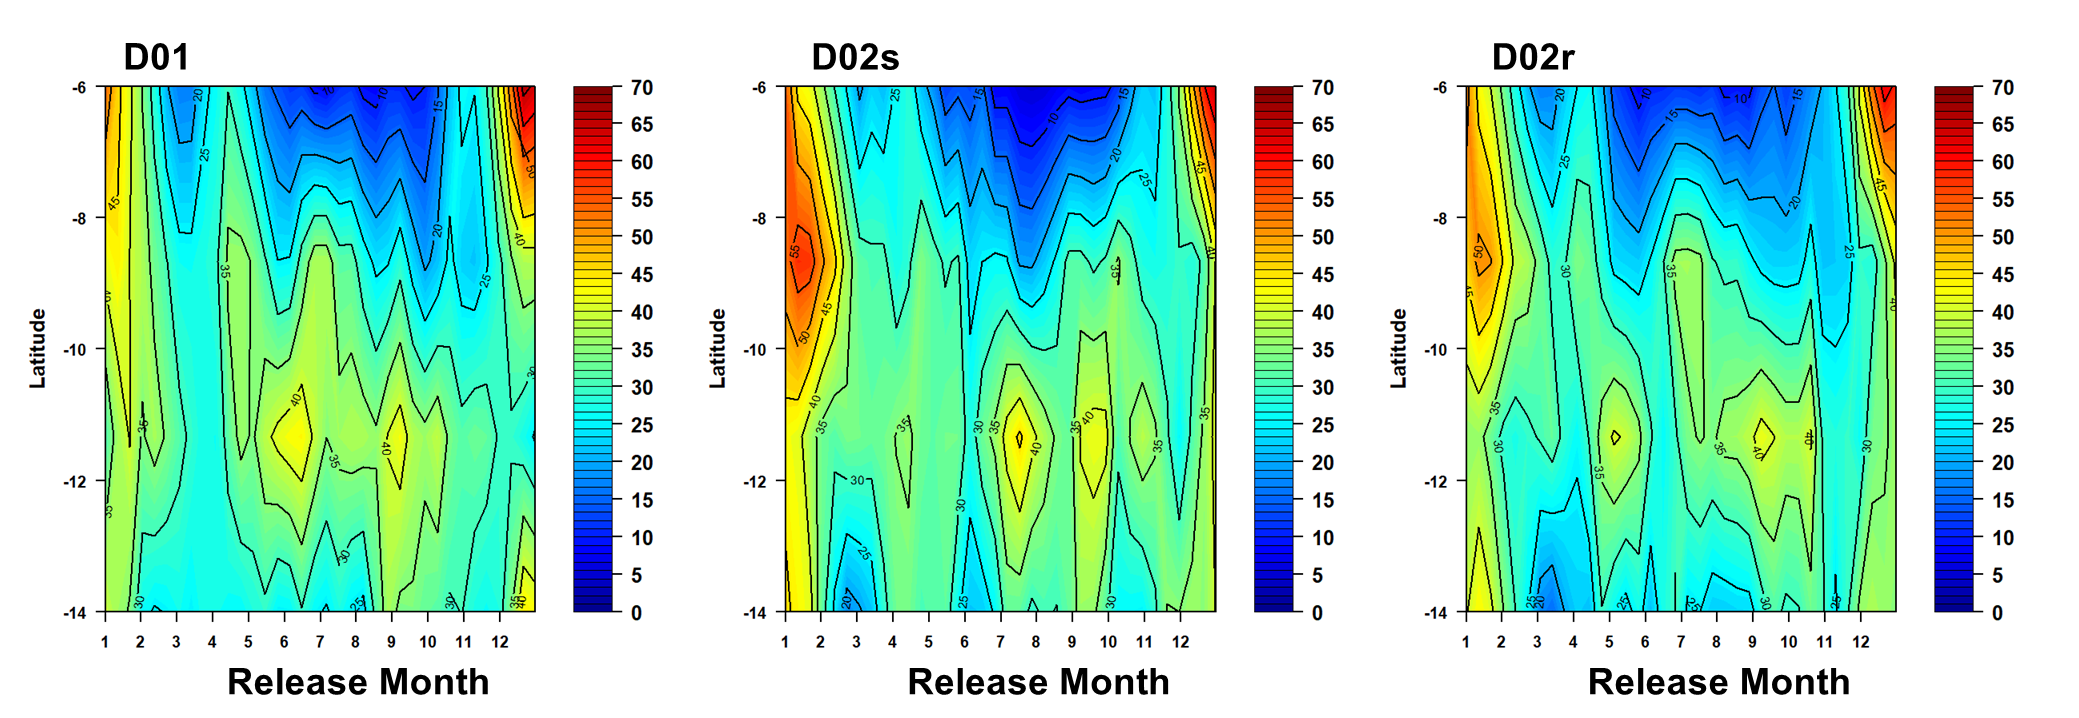
\includegraphics[width=1.0\textwidth]{figures/Chap2SpatialVariation.png}
	\centering
	\caption{Spatial variation of retention rates for simulation 1 (D01), simulation 2 (D02s) and simulation 3 (D02r).}
	\label{Chap2SpatialVariation}
\end{figure}
\end{center}

Fig. \ref{Chap2CoastlineBehavior} describes the interaction between release bathymetry and coastline behavior. Only in the area closest to the coast (0 - 100 m of bathymetry) the beaching coastline behavior had a significant effect in simulation 1 (D01), simulation 2 (D02s) and simulation 3 (D02r). The other 2 coastlines behaviours had not an important effect.\\

\begin{figure}[ht]
	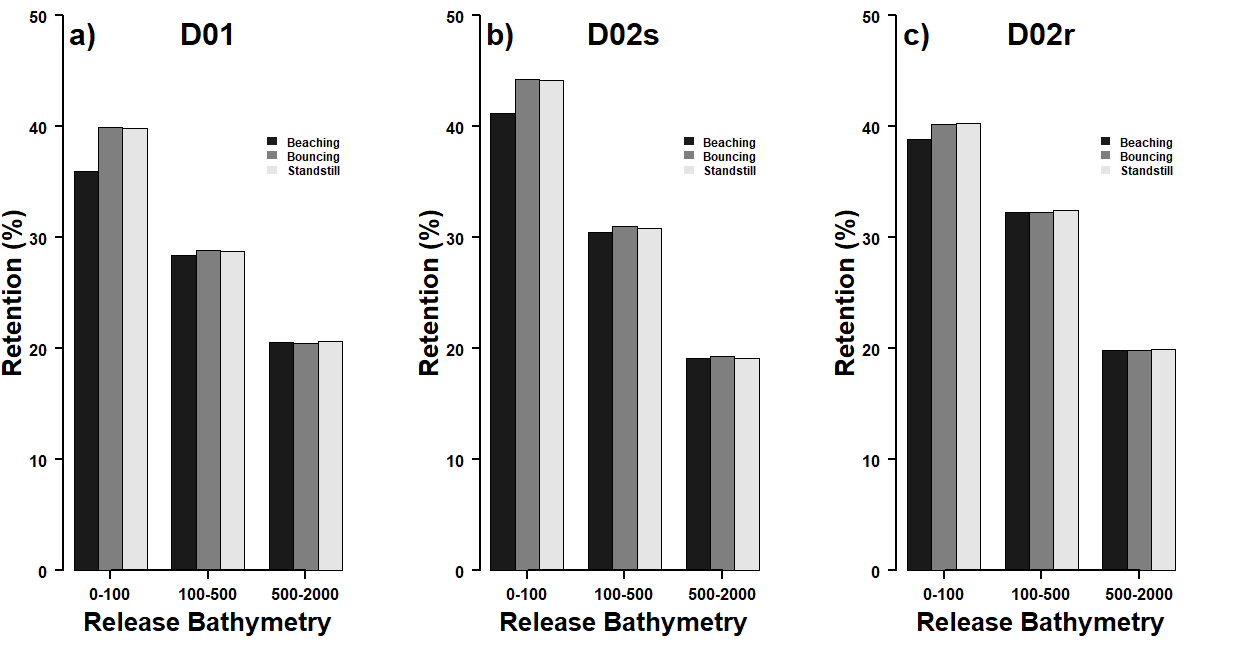
\includegraphics[width=1.0\textwidth]{figures/Chap2CoastlineBehavior.png}
	\centering
	\caption{Barplots of retention rates as a function of coastline behavior and release bathymetry for simulation 1 (D01), simulation 2 (D02s) and simulation 3 (D02r).}
	\label{Chap2CoastlineBehavior}
\end{figure}

\clearpage

\section{Discussion}\label{Chap2Disc}

A sensitivity analysis to spatial resolution, bathymetry and coastline behavior was applied to the retention rates off Peru using \gls{ich} model, a powerfull Lagrangian tool \citep{LettVerl2008}. This tool allowed us to track virtual particles in a 3D environment and to know the location of each particle at each time step.\\

The fact that there was no significant difference between simulation 1 (D01), simulation 2 (D02s) and simulation 3 (D02r) strengthen the conclusions found by \citep{BrocLett2008} who used a spatial resolution forcing only slightly greater than 10 km, despite their study had a wider latitudinal range (2º - 20º S) than the one used in this chapter (6º - 14º S). \cite{BrocLett2008} also found that release depth is the most important factor (22.7 \% of explained variance) although in a smaller proportion than in the present chapter (30.11 \%). However, \cite{BrocLett2008} found that the next most important factors were release latitude (7.2 \%) and then release bathymetry (3.9 \%), in contrast to the present chapter in which release latitude (4.58 \%) was less important than release bathymetry (12.95 \%). Concerning the release bathymetry, finding a higher value of percentage of variance explanation in this chapter compared to \cite{BrocLett2008}, could be due to the topographic sources \citep{SmitSand1997} used by them and the one used in the present chapter \citep{BeckSand2009} to represent the bathymetry, which could provide a better description of the seafloor and affect circulation and retention structures also affecting retention rates as \cite{RojaLand2014} reported.\\

\cite{LettPenv2007} applied Lagrangian simulation experiments to evaluate the processes of enrichment, retention and concentration proposed as the mechanisms that favor the recruitment of marine species \citep{Baku1998, Baku2010}. \cite{LettPenv2007} showed that after 20 days of drifting, the zones of highest retention were located between grade 10\textdegree S - 14\textdegree S, similar to our results in the 3 simulations, values that were constant throughout the year in this latitudinal range, even though retention was calculated after 30 days of drift. \cite{LettPenv2007} also showed a general seasonal pattern with the summer months favoring retention as well as in this chapter, however, we can now know that retention is highly dependent on initial depth (release depth), in agreement with \cite{BrocLett2008}, therefore, the larval retention of any species will depend on its spawning depth or its vertical behaviour \citep{OspiPara2012}.\\

A spatial resolution analysis was applied in the Humboldt ecosystem for one mollusk species \citep{GaraKapl2014}. Between 3 km and 7.5 km hydrodynamic forcings, no difference in dispersion distance was observed, however, both experiments also demonstrated that the closer to coast, the greater the success of the individuals, in this case called larval settlement (and retention in this chapter). It should be noted that they used much longer drift times (80 days and 140 days).\\

Something that was not evaluated in this work was the effect of wind forcing frequency (monthly winds and daily winds) at high resolution (2 km, D02), which results in increased retention rates while maintaining patters patterns although this was applied in very coastal and small areas at the level of a bay \citep{FlorTam2019}.\\

This could have implications when we use different coastline behaviors, as demonstrated in this chapter, in which only beaching behavior in areas very close to the coast (0 - 100 m) had significant impacts on retention rates, although did not have a major impact at level of the continental shelf off Peru, could have a significant effect if we study problems such as oil spills or accumulation of microplastics on the coast \citep{AtwoFalc2019,LopeNajj2021}.\\

Finally, we can conclude that to work on \textit{\gls{ringens}} recruitment simulations, in order to save computational time and energy, we can continue with a spatial resolution of 10 km. In addition, it is recommended to use the coastal behaviour called standstill, since for the purposes of our research it will not significantly affect near-shore particle transport.\\

\clearpage